\subsection{Simple Manufacturing Cell \label{ss:prmpc}}
We illustrate the construction of a timed transition model for a CAN-based
system using the example of a simple manufacturing cell which has been
discussed in~\cite{bjh:96}. Figure~\ref{fig:mpcpic} is a graphical
representation of the system. A production process, outside the cell,
continually deposits items at position 1 of the producer conveyor belt.  The
producer belt controller drives the belt to move items from position 1 to
position 2. The robot controller captures each item at position 2, rotates and
processes the item. After processing, the robot rotates again and attempts to
deposit the item on the consumer conveyor belt at position 3. The consumer
belt controller operates the belt to move items from position 3 to position 4
where they are removed by some external consumption process. We outline an
implementation in which the three controlling processes are physically
distributed. They interact with the environment using sensors and actuators,
and communicate with each other via a CAN.

\begin{figure}
\begin{center}
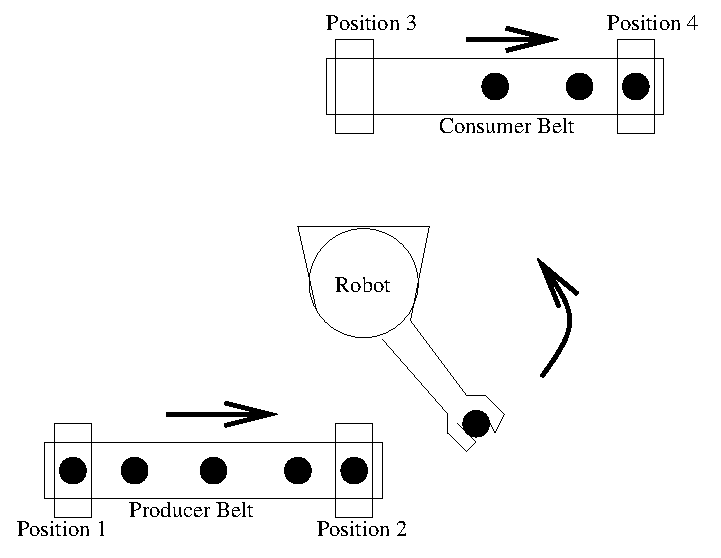
\includegraphics[width=.5\linewidth]{PRACTICE/prodcell.eps}
\end{center}
\caption{Simple Manufacturing Cell\label{fig:mpcpic}}
\end{figure}
 
Figures~\ref{fig:pbc},\ref{fig:rc} and \ref{fig:cbc} show the main details of
implementations of controllers for the producer belt, robot and consumer belt,
respectively.  This example informally introduces an Ada-like system
description language, \candle, which is more suitable for use by developers than
the language of the previous section, \bcandle, in describing complex broadcasting
real-time systems.  \candle\ is given a formal semantics in terms of timed
transition systems by translation into \bcandle.

The manufacturing cell is implemented by three distributed processes which execute
in parallel and communicate via a CAN. They interact with the environment using
a variety of sensors and actuators. Environmental interaction is modelled and
implemented by simple sequential operations ({\tt CheckPosition2, BeltOn,
DepositItem} etc.) which are usually analysed independently to obtain
bounds on performance. It is assumed that sensors and actuators are  
not shared but that each is controlled directly by a single task; other processes
which desire access to a sensor/actuator must communicate their intentions
to the controlling task by sending a CAN message.
 
\begin{figure}
\scriptsize
\begin{verbatim}
task ProducerBelt with data ProducerBelt
using
  constant PRODPERIOD
  var p1, p2, belton
  op CheckPosition1, CheckPosition2, BeltOn, BeltOff
is
  every PRODPERIOD do
    CheckPosition2;
    snd(pos2,p2);
    if p2 and belton then BeltOff end_if;
    CheckPosition1;
    if p1 and not (p2 or belton) then BeltOn end_if
  end_every
end_task
\end{verbatim}
\caption{Producer Belt Controller \label{fig:pbc}}
\end{figure}

\begin{figure}
\scriptsize
\begin{verbatim}
task Robot with data Robot
using
  var p2, p3 
  op ExtendArm, RetractArm, 
     CaptureItem, DepositItem,
     RotateA_90, RotateC_180
is
  loop do
    rcv(pos2,p2);
    if p2 then
      ExtendArm; CaptureItem; RetractArm;
      RotateA_90;
      ExtendArm; ProcessItem; RetractArm;
      RotateA_90;
      loop RELEASE do
        rcv(pos3,p3);
        if not p3 then
          ExtendArm; DepositItem; RetractArm;
          exit RELEASE
        end_if
      end_loop;
      RotateC_180
    end_if
  end_loop
end_task   
\end{verbatim}
\caption{Robot Controller\label{fig:rc}}
\end{figure}


\begin{figure}
\scriptsize
\begin{verbatim}
task ConsumerBelt with data ConsumerBelt
using
  constant CONSPERIOD 
  var p3, p4, belton
  op CheckPosition3, CheckPosition4, BeltOn, BeltOff
is  
  every CONSPERIOD do
    CheckPosition4;
    if p4 and belton then BeltOff end_if
    CheckPosition3;
    snd(pos3,p3);
    if p3 and not (p4 or belton) then BeltOn end_if
  end_every
end_task 
\end{verbatim}
\caption{Consumer Belt Controller\label{fig:cbc}}
\end{figure}

The producer belt controller is a periodic task. It maintains three boolean
variables {\tt p1, p2\/} and {\tt belton\/} to model the external
environment. {\tt p1\/} and {\tt p2\/} are updated by {\tt CheckPosition1\/}
and {\tt CheckPosition2\/}, respectively, and are set to {\tt true\/}
(resp. {\tt false\/}) when the corresponding position sensor indicates the
presence (resp. absence) of an item at its position. {\tt belton\/} is updated
by {\tt BeltOn\/} and {\tt BeltOff\/} in the expected way. Each period, the
belt controller interacts with a belt sensor to check if an item has reached
position 2. It broadcasts the sensor value on the CAN. If there is an item at
position 2 and the belt is moving, then an actuator is triggered to turn the
belt off.  If an item is placed in position 1 when the belt is off and there
is no item at position 2, the controller turns the belt on. The behaviour of
the consumer belt controller is similar.

The robot controller is an event-driven task. Repeatedly, it waits to receive
a CAN message from the producer belt controller, which indicates the presence
or absence of an item in position 2.  When it detects the presence of an item,
it actuates the robot to capture and process it, extending and retracting the
robot arm and rotating the robot as necessary. Following processing, the robot
controller seeks to deposit the processed item onto the consumer belt. It does
so by repeatedly receiving CAN messages, from the consumer belt, regarding the
status of position 3. When it receives a message indicating that there is no
item at position 3, it causes the robot to deposit the processed item and to
return to its original position.

Processes communicate using a single communication channel which carries two
types of message, position 2 and position 3 status messages, distinguished by
the message identifiers {\tt pos2\/} and {\tt pos3\/}. A task which wishes to
communicate either by sending or receiving a message makes the necessary
system call ({\tt snd\/} or {\tt rcv\/}) with parameters which denote the
message identifier and the data variable for the message data value.

As discussed in section~\ref{sec:bcdata}, the specification and
implementation of the data environment for each task, and the operations which
they can perform upon it, are expressed in a language of the developer's
choice. We currently use B~\cite{abr:96} for specification and C for
implementation. Data clauses in \candle\ (such as {\tt with data ProducerBelt})
make the links to the appropriate specifications and implementations from
which a description of the effect of the state transformers, and the bounds
upon their performance, can be obtained.

\subsubsection{Constructing a timed transition model}  
Figure~\ref{fig:mpcbc} shows the initial task state which is constructed
for the manufacturing cell. 
The processes interact with the environment using a
variety of sensors and actuators. Environmental interaction is modelled and
implemented by simple data operations ({\tt CheckPosition2, BeltOn,
DepositItem} etc.) which are analysed independently to obtain bounds on
performance.  The notation \verb'[CheckPosition2]' etc. is used throughout to
abbreviate \verb'[CheckPosition2:t1,t2]' where {\tt t1} and {\tt t2} are the
lower and upper bounds, respectively, on the execution time of the code which
implements \verb'CheckPosition2'.  Other computations
(e.g. \verb'[pre_timer]', \verb'[jump]' etc.) leave the data environment
unchanged and are assumed to take some positive amount of time to execute.
Each task maintains a number of boolean variables (e.g. {\tt p1, belton\/}) to
model the state of the external environment; these variables are updated by
the execution of one of the data operations (e.g. \verb'CheckPosition1',
\verb'BeltOff'). The variable \verb'__exit_RELEASE' is updated by
\verb'[PRE_EXIT_RELEASE]' and \verb'[POST_EXIT_RELEASE]' and is tested by the
predicate \verb'exit_RELEASE'.  It allows the modelling of a simple loop with
an exit condition.  Processes communicate using a single communication channel
which carries two types of message, position 2 and position 3 status messages,
distinguished by the message identifiers {\tt pos2\/} and {\tt pos3\/}. The
static attributes of the channel are given in the network section of the
system model. Initially, the channel queue is assumed to be empty and the
status to be \emph{free}.

\begin{figure}
\scriptsize
\begin{verbatim}
PBelt | Robot | CBelt
where
PBelt = 
   [pre_timer] ; 
   ([CheckPosition2]; 
    [pre_snd]; k!pos2.p2; [post_snd];
    [eval_guard1]; 
    (guard1 -> [BeltOff] + not_guard1 -> [branch]);
    [CheckPosition1]; 
    [eval_guard2]; 
    (guard2 -> [BeltOn] + not_guard2 -> [branch]); 
    idle) [> 
   [approx_PRODPERIOD]; [post_timer]; [jump]; PBelt

Robot =
  [pre_rcv]; k?pos2.p2; [post_rcv];
  [eval_guard3]; 
  (guard3 -> 
    [CaptureProcessRotate]; 
    (Release [> exit_RELEASE ->[POST_EXIT_RELEASE]);
    [RotateC_180] 
  + notguard3 -> [branch]); [jump]; Robot

Release =
  [pre_rcv]; k?pos3.p3; [post_rcv]; 
  [eval_guard4] ; 
  (guard4 -> [Deposit]; [PRE_EXIT_RELEASE]; idle 
  + notguard4 -> [branch]); 
  [jump]; Release

CBelt =
  [pre_timer];
  ([CheckPosition4]; [eval_guard5];
   (guard5 -> [BeltOff] + notguard5 -> [branch]); 
   [CheckPosition3]; 
   [pre_snd]; k!pos3.p3; [post_snd];
   [eval_guard6]; 
   (guard6 -> [BeltOn] + not_guard6 -> [branch]); 
   idle) [> 
  [approx_CONSPERIOD]; [post_timer]; [jump]; CBelt

/*  Abbreviations
guard1 == PBelt.p2 and PBelt.belton   
guard2 == PBelt.p1 and not (PBelt.p2 or PBelt.belton)
guard3 == Robot.p2     guard4 == not Robot.p3
guard5 == CBelt.p4 and CBelt.belton   
guard6 == CBelt.p3 and not (CBelt.p4 or CBelt.belton)

not_guardn == not guardn
*/

network
  /*          pri  dlb  dub  dlB  duB         */
  k = (pos2:    1,  43,  53,  10,  12;  
       pos3:    2,  43,  53,  10,  12)

data
  PBelt.p1 = false; PBelt.p2 = false;
  Robot.p2 = false; Robot.p3 = false; 
  CBelt.p3 = false; CBelt.p4 = false; 
  PBelt.belton = false; CBelt.belton = false;
  __exit_RELEASE = false
\end{verbatim}
\caption{\bcandle\ model of Manufacturing Production Cell \label{fig:mpcbc}} 
\end{figure}
